\subsection{Aclaraciones}
En todos lo experimentos, para cada tamaño de secuencia se corrió el programa 50 veces, guardando el tiempo de cada ejecución. Para elegir el valor mas representativo de la muestra tomo la \textbf{media} de cada tamaño. La media es lo que puede verse en el gráfico. \\

La generación de secuencias aleatorias de tamaño $n$ fue hecho en Python3 usando: 
\begin{center}
\begin{tabular}{c}
\begin{lstlisting}[language=Python]
[random.randrange(cota_superior) for _ in range(n)]
\end{lstlisting}
\end{tabular}
\end{center}

donde $cota\_superior$ es un número lo suficientemente grande para que no condicione la muestra. En el gráfico, el valor usado como cota es 1000000.

\subsection{Aleatorias}

Podemos observar una clara diferencia entre los algoritmos de backtracking y los algoritmos de programación dinámica. Esto es lo esperado si tenemos en cuenta que en nuestro análisis original concluímos que los primeros tenían complejidad \textbf{exponencial}, mientras que los segundos tenían complejidad \textbf{polinomial}. \\

{\centering
  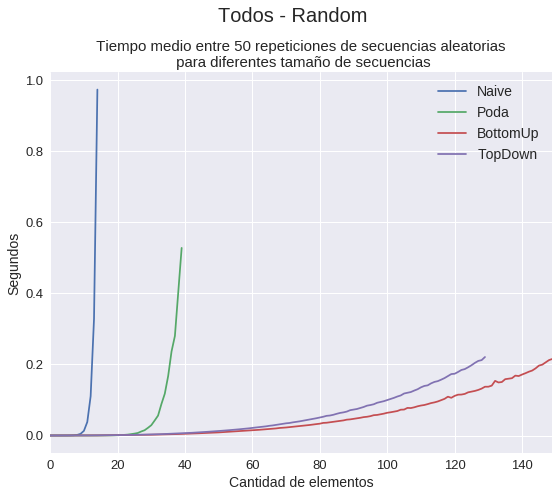
\includegraphics[width=0.75\textwidth]{informe/img/experimentos/todos-random.png} \\
} 

Era esperable que el algoritmo con \textit{poda} sea mucho mas eficiente que el algoritmo \textit{naive}, pero veamos que pasa con los de programación dinámica: \\

{\centering
  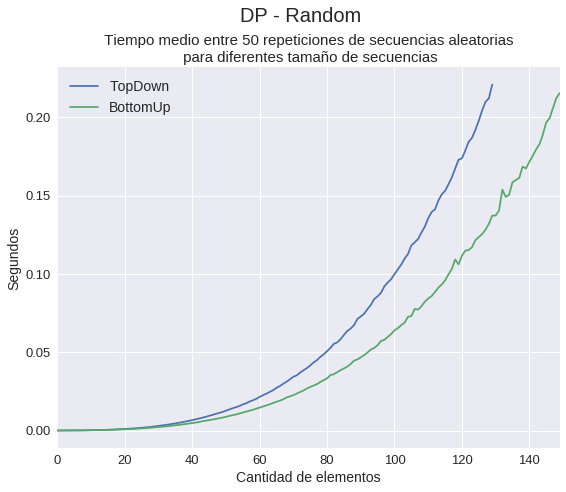
\includegraphics[width=0.70\textwidth]{informe/img/experimentos/dp-random.png} \\
}
\hspace{1\textwidth} \\